%\documentclass[a4paper,12pt]{report}
\documentclass[12pt]{uafthesis}


%allows for hyperlink
\usepackage{hyperref}
%re-define how \autoref (found in hyperref package) prints a chapter reference
%Default is "chapter", but I want "Chapter" instead
\renewcommand*{\chapterautorefname}{Chapter}
%\usepackage{url}

%allows for degree symbol, among other things presumably
\usepackage{textcomp}

%draws bounding boxes around the major page elements. For troubleshooting
%\usepackage[showframe]{geometry}

%Allows for drawing circuit diagrams
%\usepackage[siunitx]{circuitikz}
\usepackage{circuitikz}

%allows multiple rows in a single column withing a table
\usepackage{multirow}

\usepackage{amsmath, amssymb, amsfonts} % Thanks, AMS!
\usepackage{fixltx2e} % Allows \(\) in captions, amongst other things.
%\usepackage{ppl} % The Paladino font (tough to find?)
\usepackage{pxfonts} % Paladino-like fonts
\usepackage{graphicx, float} % Graphics stuff
\usepackage{verbatim} % Mostly for the comment environment.
%\usepackage{chapterbib} % This is an option for those bundling papers.
%\usepackage[square]{natbib}
%\usepackage{tocbibind} % This fixes the "bibliography in ToC" problem.
                        % Use with chapterbib.



%certain default hyphenations aren't what I want
\hyphenation{geo-ther-m-al}

%Various title/signature page info
\author{Nathan Green}
\title{Optimal Grid Architecture for Power Generation and Distribution in Hybrid Microgrids with Geothermal Organic Rankine Cycle Turbine and Diesel Electric Generators}

\degreeyear{2018}
\degreemonth{}
\degree{Master of Science}
\department{Dept. of Electrical Engineering}
\numberofmembers{3} % Make sure this is right! The grad school hates empty
                    % signature lines.
\committeewidth{4in}
\approvedwidth{4in}
\comitteespace{\hfill}
\approvedspace{\hfill}

\prevdegrees{B.S.}
\college{College of Engineering and Mines}

\begin{document}

\makesig
\maketitle

\begin{abstract}

Diesel electric generation is heavily used in remote permanently islanded microgrids, even in areas where alternative resources are readily available. The cost of diesel fuel for these generators is high in part because of the high cost of transportation to these distant sites using vehicles that rely on some form of petroleum themselves. 
%Additionally, as the cost of fuel increases, so too does the cost of transportation, hitting these remote communities harder. 
This thesis will show that local resources such as geothermal hot springs can provide primary power for these remote microgrids, even at relatively low temperatures below the boiling point of water. The geothermal heat will be converted to electrical energy using an organic Rankine cycle turbine in combination with a self-excited induction generator. A steady-state energy balance model will be developed using MATLAB Simulink to simulate greenfield and brownfield geothermal microgrids at Pilgrim Hot Springs, Alaska and Bergsta$\eth$ir, Iceland, respectively, to demonstrate viability of this microgrid design. 
The results of the simulations have shown modest loads can be primarily powered off of these low temperature geothermal organic Rankine cycles over long time scales. As expected, more power is available during colder months when sink temperatures are lower. More research should be done to examine system response over shorter time scale transients, which are not covered in the scope of this work.

%A stability analysis will be conducted using the long and short term simulation models which evaluate system voltage and frequency under different conversion topologies. A cost analysis will also be conducted to compare the economic viability of operating the different systems in remote communities. It is expected the system with greatest stability will not be the most cost-effective, but that there is a system which provides stable power within reasonable tolerances at optimal cost.

\end{abstract}


%Table of Contents and such
\tableofcontents
\listoffigures
\listoftables
%\listofothermaterials
%\listofappendices

%Each chapter is included
\chapter{Introduction}

\section{Problem Statement}
The state of Alaska currently has dozens of communities which are electrically isolated from the rest of the state. They effectively act as remote permanently islanded microgrids. These communities typically use diesel generators to provide most of their electrical power. Power sources such as coal or natural gas are less expensive in larger grids but these microgrids are too small to take advantage of such economies of scale. This makes it expensive to operate relative to the size of the communities.

One method of reducing operating costs is to offset diesel fuel through the usage of renewable energy resources.


\section{Microgrid Description}
Microgrids are electrical systems composed of sources and loads within a well defined electrical boundary. Energy storage is often incorporated into systems as well, but not necessarily. Many microgrids are connected to a larger grid but with the ability to become separated, or islanded, while still maintaining some or all of the loads.

A microgrid can operate using Alternating Current (AC), Direct Current (DC), or a hybridization of the two. The choise to whether to use AC or DC depends on the demands of the loads, the available power sources and conversion devices, as well as the existing electrical infrastructure.

Approximately 70\% of the population of Alaska is connected to a single grid called the Railbelt \cite{railbelt}. The Railbelt stretches over 600 miles from the Homer on the Kenai Peninsula to the greater Fairbanks area in the interior and includes most communities on the road system in between. The remaining communities and villages are effectively permanently islanded microgrids. 

\subsection{Sources}
Microgrid power is typically generated by Distributed Energy Resources (DER). This can include renewable resources such as solar photovoltaics, wind turbine generators, and geothermal as well as and non-renewable sources such diesel generators and natural gas microturbines. 

Diesel generators use the combustion of diesel fuel to spin an alternator producing AC power. These generators are prolific in rural Alaska generally being used as the prime mover to regulate grid frequency and voltage. 
%These generators are composed of an engine, alternator, fuel system, excitation system, governor, cooling system, exhaust system, and turbocharger.
Due to their widespread use, significant energy cost savings can be generated by reducing fuel consumption through efficiency improvements and use of alternate energy sources.

Geothermal generators are heat engines and can operate similarly to traditional coal and nuclear plants. Heat causes a working fluid to thermally expand and change phases thus spinning a turbine to produce AC power. The primary difference is that geothermal systems get heat from the Earth as opposed to combustion or nuclear reactions. Geothermal generators can be divided into high heat and low heat categories. High heat geothermal systems work with temperatures at and above the boiling point of water which means water can be used as the working fluid. Low heat systems operate at temperatures below the boiling point of water therefore must use a refrigerant as an alternative working fluid. 

Wind turbine generators 
%Describe distributed energy resources (DER) in general, diesel gensets, geothermal sources, and 
\begin{verbatim} 
 Address wind & solar too.
\end{verbatim}

\subsection{Loads}
Well designed microgrids are designed around expected loads. 
\begin{verbatim} 
 Describe dispatchable loads and give some examples. 
\end{verbatim}

\subsection{Storage}
Energy storage is beneficial to microgrid operation because it allows generation to be spread over time. Such devices can include batteries, flywheels, supercapacitors, pumped hydro, and more. These devices have different storage duration and discharge times making different storage technologies advantageous in different situations \cite{Schoenung2003}. The discharge of bulk energy storage over the course of many hours allows for load leveling and provides spinning reserve for the grid. Load peak shaving typically involves a discharge time from minutes to several hours. Energy storage discharge over seconds and subseconds is generally done to improve power quality.
\begin{verbatim}
 Define spinning reserve somewhere
\end{verbatim}

\subsection{Control}
A microgrid control system ties all the other components together. Control systems monitor maintain voltage and frequency of the grid while ensuring sufficient active and reactive power is supplied to the loads.

\subsection{Conversion}
Conversion devices take a form of electrical power (AC or DC) and convert it into a different form. Inverters convert DC power into sinusoidal AC power. Rectifiers convert AC to DC. DC-DC converters can step up or down the voltage level of a DC power source. Transformers can step up or down the voltage level of an AC source while maintaining frequency. Modifying the frequency of an AC source typically involves rectifying the source then inverting then that output at the desired frequency.


\chapter{Energy Conversion}
\label{ch:conv}

Energy and power take many different forms, from the initial sources to the end results used. Necessarily, methods have been developed to convert the different forms of energy or power from one to another. The first method addressed in this chapter is the conversion process of thermal to mechanical to electrical energy found in heat engines and generators. This thesis is focused on geothermal heat, however heat engines can be used with a number of different sources including the burning of a fuel such as biomass or coal, or even as waste heat from an independent process. Next conversion between different forms of electrical power will be addressed.

%This file used to contain the geothermal chapter, now contains thermal/mechanical section of the conversion chapter
\section{Thermal Energy}
Thermal energy, or heat, can originate from many different sources including combustion of a fuel, radioactive decay, or absorption of light from the sun. Heat can be used directly to warm a building, but it is also a critical step in most traditional methods of generating electrical power. 
%\chapter{Geothermal Energy}
%\label{ch:geothermal}

\subsection{Enthalpy}
Enthalpy describes the energy of a system available to be converted to work. It is related to the temperature of the geothermal resource, but also dependent on the pressure and volume. Temperature is usually the primary metric of a resource, but even a high temperature source is useless without sufficient volume flow. Quantitatively enthalpy is expressed as \cite{Nellis2009}
\begin{equation}
H = U + pV
\end{equation}
where $U$ is the internal energy, which is function of temperature, $p$ is the pressure of the system, and $V$ is the volume. Generally it is more convenient to use the change in enthalpy rather than absolute values. After a system undergoes some thermodynamic process, the system will always have some remaining internal energy, pressure, and volume. Therefore, a change in enthalpy better describes the energy extracted from (or absorbed by) the system.
Additionally, the enthalpy of a system is often normalized by the its mass for comparison to other sized systems and the mass specific enthalpy, $h$, is used instead.
\nomenclature[V]{$H$}{Enthalpy of a fluid\nomunit{\si{\joule}}}
\nomenclature[V]{$U$}{Internal energy of a fluid\nomunit{\si{\joule}}}
\nomenclature[V]{$p$}{Aboluete fluid pressure\nomunit{\si{\pascal}}}
\nomenclature[V]{$V$}{Fluid volume\nomunit{\si{\meter\cubed}}}
\nomenclature[V]{$h$}{Mass specific enthalpy of a fluid\nomunit{\si{\joule\per\kilogram}}}


\subsection{Geothermal Cycles}
%%Describe each of the following but focus on cycles for low enthalpy sources
Geothermal systems can be classified as high-, medium-, or low-enthalpy\footnote{While the technical definitions differ, the terms enthalpy, heat, and temperature are often used interchangeably when qualitatively describing geothermal sources.}. Although there is no formal delineation, high-enthalpy sources generally have temperatures greater than about $150$ \textcelsius{} ($302$ \textdegree{}F) and low-enthalpy sources have temperatures lower than $100$ \textcelsius{} ($212$ \textdegree{}F) \cite{Norden2011}. Depending on the amount of extractable energy of the resource, different geothermal processes or cycles can be used to extract the maximum amount of energy from the resource.

\subsubsection{Dry Steam}
This high-enthalpy processes extracts hot steam from the earth. The steam is sent directly through a turbine then condensed into liquid water and injected back underground. 

\subsubsection{Flash Steam} 
In the flash steam process high pressure hot water is extracted then, allowed to boil becoming steam and low pressure hot water. The steam is sent through a turbine then condensed, recombined with water, and injected back underground.

\subsubsection{Binary Cycle} 
As the name implies, binary cycles involve two loops: a heat source loop and working fluid loop. Heat is collected in the heat source loop and transferred to the working loop through a heat exchanger. The working fluid then undergoes the vaporization process to spin a turbine or other type of expander. The expander is connected to a generator which converts the rotational mechanical energy into electrical energy. After some of the heat is converted, the working fluid passes through a condenser where it is cooled further. Sometimes the cooling process involves drawing in air at ambient temperature, but it can also involve a third loop. The fluids within each of the cycles must be moved using pumps. The pumps themselves need to be powered and act as a parasitic load to the system.

Binary cycles are not limited to low or medium enthalpy heat sources. The most common binary cycle is the Rankine Cycle. A diagram of the process can be seen in \autoref{fig:rankine_cycle_diagram}. In an ideal Rankine Cycle heat is added to the working fluid under high pressure to change its phase from liquid to gas. The fluid expands isentropically\footnote{In thermodynamics, isentropic processes do not have a net change in entropy.} which rotates the generator shaft, causing the fluid's temperature and pressure to drop. Additional heat is then expelled from the fluid as it condenses at a constant low pressure side of the system. Finally the fluid is isentropically pumped back to the high pressure and the process begins again.
\begin{figure}[h]
	\centering

	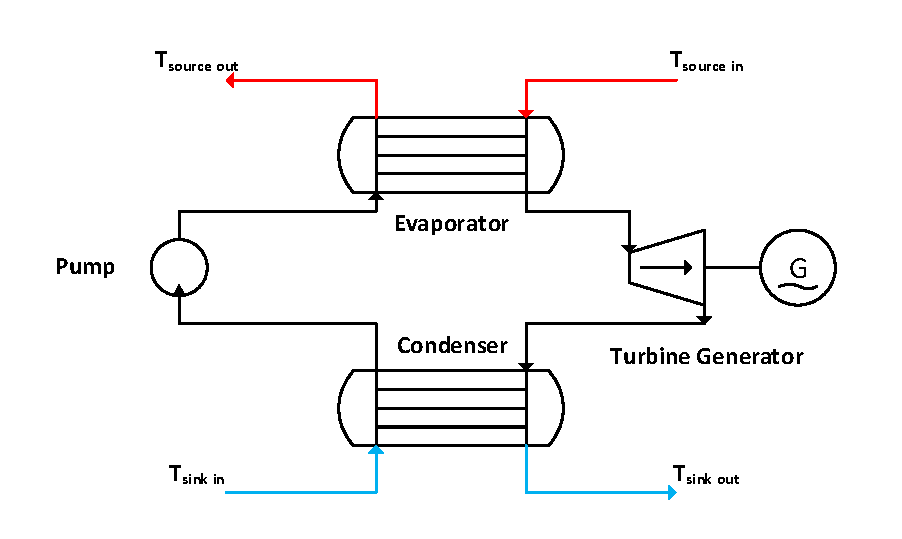
\includegraphics[width=\textwidth]{figures/RankineCycleDiagram.pdf}

	\caption{Diagram of a Rankine cycle system.}
	\label{fig:rankine_cycle_diagram}
	
\end{figure}

For geothermal sources, generally high enthalpy systems can be implemented directly with a single loop using the flash or dry steam processes. However, for lower enthalpy systems, water cannot be used as a working fluid because the temperatures are not high enough to vaporize it. In these cases an organic Rankine cycle, which uses an organic working fluid such as refrigerants instead of water, can be employed. Working fluids are typically selected for relatively low vaporization temperatures, but the thermodynamic states of the heat source must also be considered. The selection of the type of expander and pumps are discussed in Kreider \cite{Kreider}. Generally larger diameter expanders operate at lower speeds.




%\subsection{Pilgrim Hot Springs}
%Do this in 1st chapter not conv/geotherm chapter
%More thourough description of the resource and potential development plans.

 %used to contain geothermal chapter, now contains thermal section

\section{Electric Conversion}

%\subsection{Linear Power Supplies}
%Linear

%\subsection{Switched Mode Power Supplies}

\subsection{PWM vs PFM}

\subsection{DC-DC}
recent developments

\subsection{Rectifiers}
recent developments

\subsection{Inverters}
recent developments

%%This file used to contain the geothermal chapter, now contains thermal/mechanical section of the conversion chapter
\section{Thermal Energy}
Thermal energy, or heat, can originate from many different sources including combustion of a fuel, radioactive decay, or absorption of light from the sun. Heat can be used directly to warm a building, but it is also a critical step in most traditional methods of generating electrical power. 
%\chapter{Geothermal Energy}
%\label{ch:geothermal}

\subsection{Enthalpy}
Enthalpy describes the energy of a system available to be converted to work. It is related to the temperature of the geothermal resource, but also dependent on the pressure and volume. Temperature is usually the primary metric of a resource, but even a high temperature source is useless without sufficient volume flow. Quantitatively enthalpy is expressed as \cite{Nellis2009}
\begin{equation}
H = U + pV
\end{equation}
where $U$ is the internal energy, which is function of temperature, $p$ is the pressure of the system, and $V$ is the volume. Generally it is more convenient to use the change in enthalpy rather than absolute values. After a system undergoes some thermodynamic process, the system will always have some remaining internal energy, pressure, and volume. Therefore, a change in enthalpy better describes the energy extracted from (or absorbed by) the system.
Additionally, the enthalpy of a system is often normalized by the its mass for comparison to other sized systems and the mass specific enthalpy, $h$, is used instead.
\nomenclature[V]{$H$}{Enthalpy of a fluid\nomunit{\si{\joule}}}
\nomenclature[V]{$U$}{Internal energy of a fluid\nomunit{\si{\joule}}}
\nomenclature[V]{$p$}{Aboluete fluid pressure\nomunit{\si{\pascal}}}
\nomenclature[V]{$V$}{Fluid volume\nomunit{\si{\meter\cubed}}}
\nomenclature[V]{$h$}{Mass specific enthalpy of a fluid\nomunit{\si{\joule\per\kilogram}}}


\subsection{Geothermal Cycles}
%%Describe each of the following but focus on cycles for low enthalpy sources
Geothermal systems can be classified as high-, medium-, or low-enthalpy\footnote{While the technical definitions differ, the terms enthalpy, heat, and temperature are often used interchangeably when qualitatively describing geothermal sources.}. Although there is no formal delineation, high-enthalpy sources generally have temperatures greater than about $150$ \textcelsius{} ($302$ \textdegree{}F) and low-enthalpy sources have temperatures lower than $100$ \textcelsius{} ($212$ \textdegree{}F) \cite{Norden2011}. Depending on the amount of extractable energy of the resource, different geothermal processes or cycles can be used to extract the maximum amount of energy from the resource.

\subsubsection{Dry Steam}
This high-enthalpy processes extracts hot steam from the earth. The steam is sent directly through a turbine then condensed into liquid water and injected back underground. 

\subsubsection{Flash Steam} 
In the flash steam process high pressure hot water is extracted then, allowed to boil becoming steam and low pressure hot water. The steam is sent through a turbine then condensed, recombined with water, and injected back underground.

\subsubsection{Binary Cycle} 
As the name implies, binary cycles involve two loops: a heat source loop and working fluid loop. Heat is collected in the heat source loop and transferred to the working loop through a heat exchanger. The working fluid then undergoes the vaporization process to spin a turbine or other type of expander. The expander is connected to a generator which converts the rotational mechanical energy into electrical energy. After some of the heat is converted, the working fluid passes through a condenser where it is cooled further. Sometimes the cooling process involves drawing in air at ambient temperature, but it can also involve a third loop. The fluids within each of the cycles must be moved using pumps. The pumps themselves need to be powered and act as a parasitic load to the system.

Binary cycles are not limited to low or medium enthalpy heat sources. The most common binary cycle is the Rankine Cycle. A diagram of the process can be seen in \autoref{fig:rankine_cycle_diagram}. In an ideal Rankine Cycle heat is added to the working fluid under high pressure to change its phase from liquid to gas. The fluid expands isentropically\footnote{In thermodynamics, isentropic processes do not have a net change in entropy.} which rotates the generator shaft, causing the fluid's temperature and pressure to drop. Additional heat is then expelled from the fluid as it condenses at a constant low pressure side of the system. Finally the fluid is isentropically pumped back to the high pressure and the process begins again.
\begin{figure}[h]
	\centering

	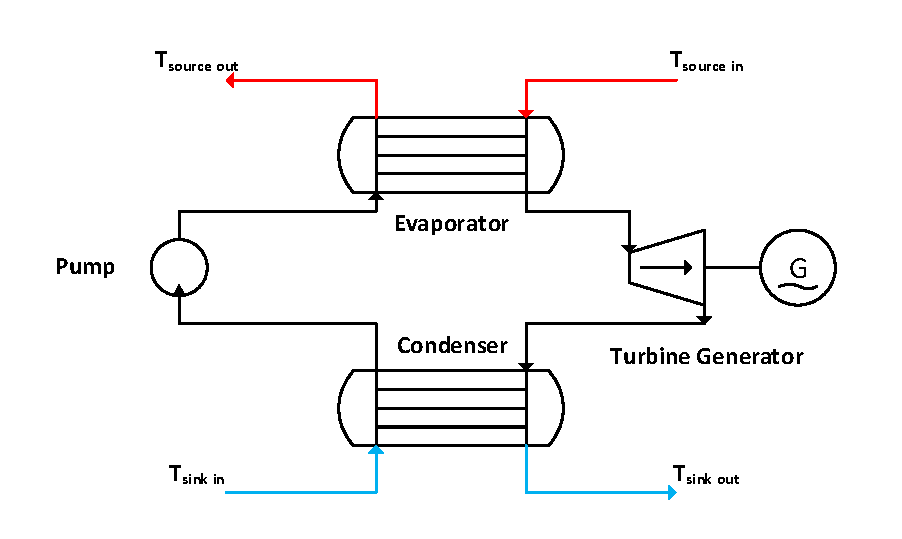
\includegraphics[width=\textwidth]{figures/RankineCycleDiagram.pdf}

	\caption{Diagram of a Rankine cycle system.}
	\label{fig:rankine_cycle_diagram}
	
\end{figure}

For geothermal sources, generally high enthalpy systems can be implemented directly with a single loop using the flash or dry steam processes. However, for lower enthalpy systems, water cannot be used as a working fluid because the temperatures are not high enough to vaporize it. In these cases an organic Rankine cycle, which uses an organic working fluid such as refrigerants instead of water, can be employed. Working fluids are typically selected for relatively low vaporization temperatures, but the thermodynamic states of the heat source must also be considered. The selection of the type of expander and pumps are discussed in Kreider \cite{Kreider}. Generally larger diameter expanders operate at lower speeds.




%\subsection{Pilgrim Hot Springs}
%Do this in 1st chapter not conv/geotherm chapter
%More thourough description of the resource and potential development plans.

	%Electronic conversion and thermal/mechanical conversion chapters combined


\bibliographystyle{ieeetr}
\bibliography{NG_bib}

\end{document}
